% !Mode:: "TeX:UTF-8"
%% Thesis Template of Yanshan University
%% for using YSUthesis package with XeLaTeX
% 2012年3月17日
%% 文档参数配置开始:
%%===========================%
\documentclass[showtypeinfo]{YSUthesis}
%  showtypeinfo 显示扉页的LaTeX版本信息,去掉即可隐藏版本信息。
%  openany      可以去掉章节起始页必须为奇数页的限制,使章节连续,不出现空白页。
%  推荐的编译顺序为:XeLaTeX > BibTeX > XeLaTeX > XeLaTeX,
%  这样可以生成正确的参考文献和交叉引用链接。

%  设置图形文件的搜索路径。支持图形格式:pdf; png; jpg.
\graphicspath{{chapter/}{figures/}}

%  执行下面的命令可以取消PDF文件中的链接颜色,使用 Adobe Acrobat Reader 查看
%  时,链接可能会有边框,但是在打印时不会出现。
%\hypersetup{colorlinks=false}

% 启用以下这段代码可以让你更改目录的缩进,以备学院有特殊要求。
%\usepackage{titletoc}
%\titlecontents{chapter}[4\ccwd]{}
%                {\bf\contentslabel{4\ccwd}}
%                {\hspace{-4\ccwd}\bf}
%                {\titlerule*[5pt]{.}\contentspage}
%\titlecontents{subsection}[68pt]{}
%                {\contentslabel{40pt}}
%                {\hspace{-4\ccwd}}
%                {\titlerule*[5pt]{.}\contentspage}

% 选择数学字体,xits-math.otf为类Times字体,Cambria Math与Office2010数学公式格式相同。
\setmathfont{xits-math.otf}
%%===========================%
%% 文档参数配置结束


%% 文档正式开始
%============================%
\begin{document}


% 以下为封面部分
%----------------------------%
  % 中文封面内容
  \classification{O441.4}                           % 中图分类号
  \UDC{537.8}                                       % UDC
  \title{燕山大学硕士学位论文\LaTeX 模板使用说明}  % 论文题目
  \author{×××}                                      % 作者姓名
  \advisor{×××教授}                                % 导师姓名
  \degree{理学硕士}                                 % 申请学位
  \major{凝聚态物理}                                % 专业
  \institute{理学院}                                % 所在单位
  \defenddate{2011年11月}                        % 答辩日期
  \school{燕山大学}                                 % 院校名称

  % 英文封面内容
  \enstatement{Science}                             % 学科或领域
  \entitle{OPTIMIZATION OF PHOTONIC CRYSTAL FIBER DISPERSION PROPERTIES USING GENETIC ALGORITHM}    % 英文题目
  \enauthor{×××}                                    % 作者英文姓名
  \enadvisor{Professor ×××}                         % 导师英文姓名
  \enschool{Yanshan University}                     % 院校英文名称
  \enathdate{2011.11}                               % 英文答辩日期

  % 生成封面
  \makecover

  % 生成中文封里
  \maketitle

  % 生成英文封里
  \makeenglishtitle

  % 生成原创性声明
  \makelicense


% 以下为前言部分
%----------------------------%
\frontmatter
\pagenumbering{Roman}

  % 摘要
  % Abstract
\clearpage
\thispagestyle{plain}
\phantomsection
\addcontentsline{toc}{chapter}{Abstract}

\centerline{\zihao{3}\bfseries Abstract}

\linespread{1.4}\zihao{-4}
\bigskip

This thesis explores the relationship between focus structure and pronoun resolution among non-native speakers of English and French. Firstly we reviewed the existing literature on the mechanism of focus effect and pronoun resolution. Then through a self-paced reading test, we find that focus, in the form of cleft structure does not necessarily increase the salience of a informational unit, thus may not in some cases make it a preferred antecedent for pronoun resolution. This result is line with previous researches on this topic. In our experiment, We also find that focused subject in French and focused object in English are processed faster, but focused subjects in both languages leads to longer response time of anaphora. Furthermore, our research also shows that the congruence between anaphora and focus does not make the latter more accessible. In this regard, we argue that the problem of whether there is subject or object preference in English and French is more complicated than the results of current studies.

\bigskip
\noindent\textbf{\zihao{4} Keywords:} 
focus effect, pronoun resolution, self-paced reading, English, French



  % 目录
  \tableofcontents
  % 表格目录
  %\listoftables
  % 插图目录
  %\listoffigures


% 以下为正文部分
%----------------------------%
\mainmatter
  \chapter{Introduction}
\label{chap:intro}

\section{What is Lorem Ipsum?}
\label{sec:apadia}

Lorem Ipsum is simply dummy text of the printing and typesetting industry. Lorem Ipsum has been the industry's standard dummy text ever since the 1500s, when an unknown printer took a galley of type and scrambled it to make a type specimen book \cite{banerjee:pedersen:2003}. It has survived not only five centuries, but also the leap into electronic typesetting, remaining essentially unchanged. It was popularised in the 1960s with the release of Letraset sheets containing Lorem Ipsum passages, and more recently with desktop publishing software like Aldus PageMaker including versions of Lorem Ipsum \cite{berment:phd:2004}.



\section{Where Does It Come From?}
\label{sec:where}

Contrary to popular belief, Lorem Ipsum is not simply random text. It has roots in a piece of classical Latin literature from 45 BC, making it over 2000 years old. Richard McClintock, a Latin professor at Hampden-Sydney College in Virginia, looked up one of the more obscure Latin words, consectetur, from a Lorem Ipsum passage, and going through the cites of the word in classical literature, discovered the undoubtable source \cite{azarova:etal:2002,budanitsky:hirst:2006}. Lorem Ipsum comes from sections 1.10.32 and 1.10.33 of ``de Finibus Bonorum et Malorum'' (The Extremes of Good and Evil) by Cicero, written in 45 BC. This book is a treatise on the theory of ethics, very popular during the Renaissance. The first line of Lorem Ipsum, ``''Lorem ipsum dolor sit amet\ldots'', comes from a line in section 1.10.32.

The standard chunk of Lorem Ipsum used since the 1500s is reproduced below for those interested. Sections 1.10.32 and 1.10.33 from ``de Finibus Bonorum et Malorum'' by Cicero are also reproduced in their exact original form, accompanied by English versions from the 1914 translation by H. Rackham. 

\begin{equation}
-\frac{(x_0 - \mu)^2}{2 \sigma^2} = -\ln 2
\end{equation}


\section{Examples}
\label{sec:examples}

The first few paragraphs of Lorem Ipsum are given below.

\subsection{First Paragraph}

Lorem ipsum dolor sit amet, consectetur adipiscing elit. Donec posuere, neque quis feugiat egestas, quam sapien dictum justo, eu vulputate nunc metus sed dui. Integer molestie leo quis libero facilisis, dictum pretium quam ornare. Vestibulum ante ipsum primis in faucibus orci luctus et ultrices posuere cubilia Curae; Vivamus luctus rutrum magna non convallis. Praesent vestibulum consequat eros, et fringilla nisi suscipit id. Nam vulputate justo dui, eu rutrum est accumsan ut. Sed molestie erat vitae mi blandit, in volutpat urna lobortis. Vestibulum mollis rutrum gravida. Fusce dolor nulla, condimentum vel pretium ut, venenatis eget leo. Ut semper placerat mauris, ut tempus est tempor vel. Interdum et malesuada fames ac ante ipsum primis in faucibus. In vitae feugiat diam. Pellentesque accumsan consequat turpis aliquam elementum.


\subsection{Next Two Paragraphs}

Vivamus dignissim arcu nunc, non aliquam sem porta vitae. Sed sodales accumsan dui sit amet egestas. Maecenas rhoncus a erat eget accumsan. 

\begin{table}[hbt!]\centering
\caption{Number of Jewels}

\begin{tabular}{l c}
\hline
Type & Quantity \\\hline
Sapphire & 6\\
Diamond & 23\\
Gold & 56\\
Silver & 235\\
Bronze & 324\\\hline
\end{tabular}
\end{table}

\begin{itemize}
\item Etiam vitae pulvinar metus, sed fringilla orci. 
\item Duis dapibus dolor risus, non ultrices enim porta sit amet. 
\item Ut eu libero augue. 
\end{itemize}

Nulla ipsum augue, feugiat ac laoreet quis, pretium ut magna. Class aptent taciti sociosqu ad litora torquent per conubia nostra, per inceptos himenaeos. Integer blandit placerat dictum.

\begin{figure}[hbt!]\centering
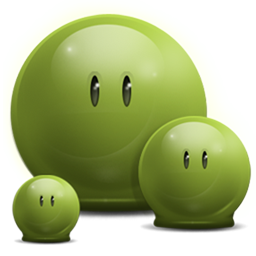
\includegraphics[width=.5\textwidth]{green}
\caption{Example figure}
\end{figure}

Sed dolor justo, scelerisque sed rutrum quis, porttitor a mauris. Cras non auctor felis, rutrum fringilla risus. Integer at convallis erat, sit amet luctus turpis. Duis sed rutrum eros, quis tempus risus. Etiam pellentesque nisi odio, eget dignissim eros ultrices et. Aliquam leo massa, fermentum vel odio sed, ullamcorper molestie lorem. Integer lorem felis, adipiscing sit amet interdum eget, auctor at lorem. Aliquam ultricies tortor eu nibh facilisis tincidunt.


\subsubsection{Some Notes}

Duis sed rutrum eros, quis tempus risus. Etiam pellentesque nisi odio, eget dignissim eros ultrices et. Aliquam leo massa, fermentum vel odio sed, ullamcorper molestie lorem.

\subsubsection{And Further}
Duis sed rutrum eros, quis tempus risus. Etiam pellentesque nisi odio, eget dignissim eros ultrices et. Aliquam leo massa, fermentum vel odio sed, ullamcorper molestie lorem.


\subsection{Least-Squares with Forgetting Factor AdaptiveLaw}

\section{Mechatronic Suspension System; History and a Brief Background}
Nulla ipsum augue, feugiat ac laoreet quis, pretium ut magna. Class aptent taciti sociosqu ad litora torquent per conubia nostra, per inceptos himenaeos. Integer blandit placerat dictum.



\section{Summary}
Nulla ipsum augue, feugiat ac laoreet quis, pretium ut magna. Class aptent taciti sociosqu ad litora torquent per conubia nostra, per inceptos himenaeos. Integer blandit placerat dictum.

Sed dolor justo, scelerisque sed rutrum quis, porttitor a mauris. Cras non auctor felis, rutrum fringilla risus. Integer at convallis erat, sit amet luctus turpis. Duis sed rutrum eros, quis tempus risus. Etiam pellentesque nisi odio, eget dignissim eros ultrices et. Aliquam leo massa, fermentum vel odio sed, ullamcorper molestie lorem. Integer lorem felis, adipiscing sit amet interdum eget, auctor at lorem. Aliquam ultricies tortor eu nibh facilisis tincidunt.
  % !Mode:: "TeX:UTF-8"
\chapter{插图}
\label{chap:figures}

插图主要涉及到:单个居中图形;两个并排图形;两个以上的并排或者堆叠的图形;图题;图形的引用;

\section{单个居中图形}

大多数情况下,需要插入的图形是单个的时候可以使用如下环境:

\begin{verbatim}
\begin{figure}[hptb]
 \centering
 
\includegraphics[width=6cm]{ysulogo}
 \caption{单个居中图形}\label{ysulogo}
\end{figure}
\end{verbatim}

其中的参数“[width=6cm]”指定图形的宽度6 cm。最后的效果如图\ref{ysulogo}所示。
\begin{figure}[hptb]
 \centering
 
\includegraphics[width=6cm]{ysulogo}
 \caption{单个居中图形}\label{ysulogo}
\end{figure}

\section{两个并排图形}
下列代码在文中插入两个并排的图形。它使用了一个称作minipage
的环境。在同一行插入两个并排的minipage,每个minipage包含一
个图形。图中minipage的参数“[0.5$\backslash$linewidth]”指定minipage
的宽度是当前正文页面的0.5倍(一半)。而插图命令中的参数
“[width=$\backslash$textwidth]”则是指定插图的宽度为当前minipage的宽
度。如果这个插图命令是在minipage环境外边的话,参数中的
“$\backslash$textwidth”的宽度为当前正文页面的宽度。
\begin{verbatim}
\begin{figure}[hptb]
  \centering
  \begin{minipage}[t]{0.5\linewidth}
    \centering
    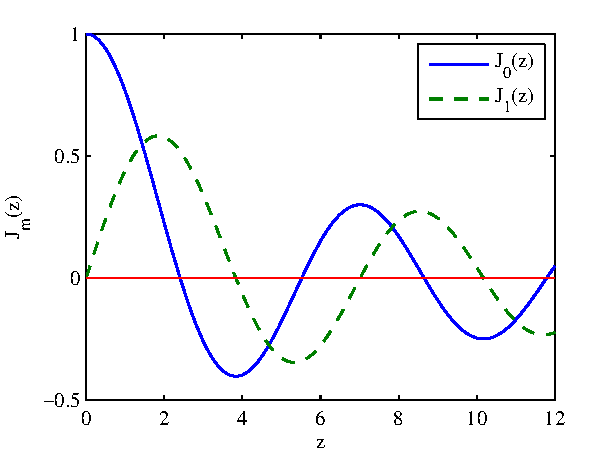
\includegraphics[width=\textwidth]{chp-2_bessel_j}
  \end{minipage}%
  \begin{minipage}[t]{0.5\textwidth}
    \centering
    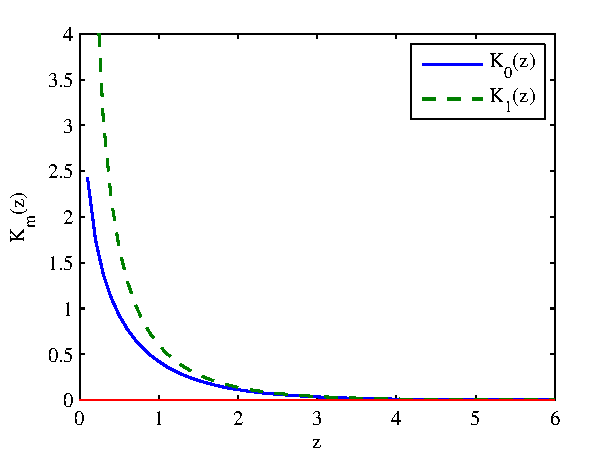
\includegraphics[width=\textwidth]{chp-2_bessel_k}
  \end{minipage}
    \caption{两个并排图形}\label{fig-dbfig}
\end{figure}
\end{verbatim}
最终结果如图\ref{fig-dbfig}所示。
\begin{figure}[hptb]
  \centering
  \begin{minipage}[t]{0.5\linewidth}
    \centering
    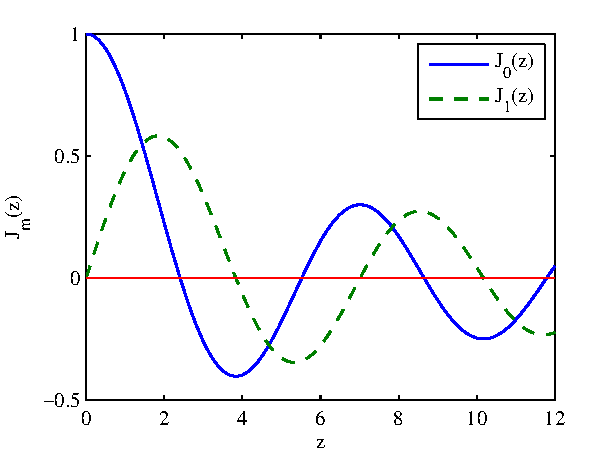
\includegraphics[width=\textwidth]{chp-2_bessel_j}
  \end{minipage}%
  \begin{minipage}[t]{0.5\textwidth}
    \centering
    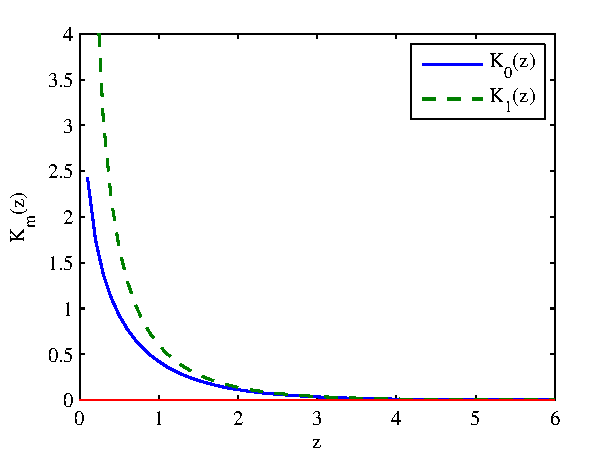
\includegraphics[width=\textwidth]{chp-2_bessel_k}
  \end{minipage}
    \caption{两个并排图形}\label{fig-dbfig}
 \end{figure}

\section{两个以上的并排或者堆叠的图形}
同样是使用minipage的方法,只不过排列的方式不同。例如4幅堆叠排列的图形。
\begin{verbatim}
\begin{figure}[hptb]
  \centering
  \begin{minipage}[t]{0.5\linewidth}
    \centering
    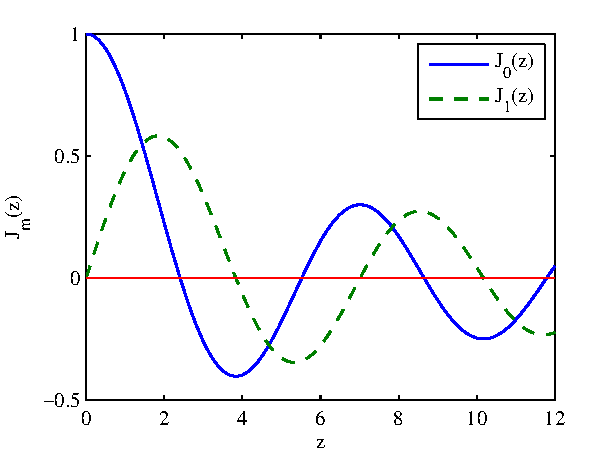
\includegraphics[width=\textwidth]{chp-2_bessel_j}
  \end{minipage}%
  \begin{minipage}[t]{0.5\textwidth}
    \centering
    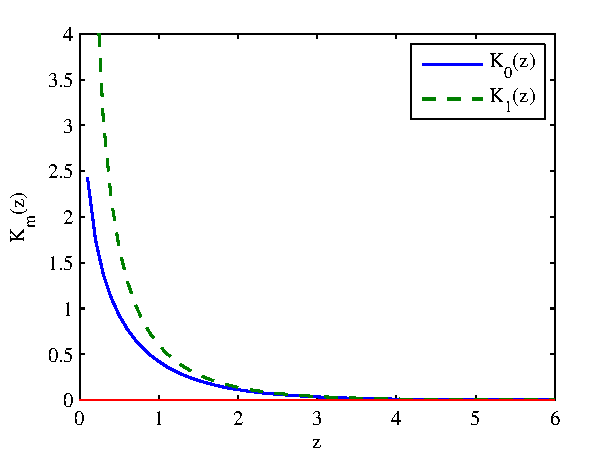
\includegraphics[width=\textwidth]{chp-2_bessel_k}
  \end{minipage}  \\
  \begin{minipage}[t]{0.5\textwidth}
    \centering
    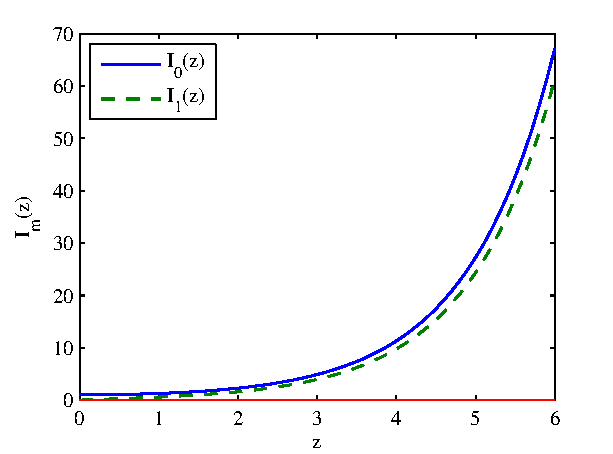
\includegraphics[width=\textwidth]{chp-2_bessel_i}
  \end{minipage}%
  \begin{minipage}[t]{0.5\textwidth}
    \centering
    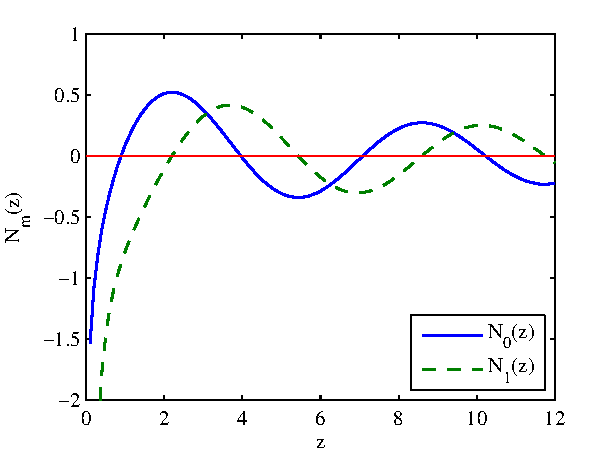
\includegraphics[width=\textwidth]{chp-2_bessel_n}
  \end{minipage}
\caption{贝塞尔函数}  \label{fig-bessel-function}
\end{figure}
\end{verbatim}
注意其中与一对并排图形不同的地方,加入了换行命令“$\backslash\backslash$”。
最终效果如图\ref{fig-bessel-function}所示。
\begin{figure}[hptb]
  \centering
  \begin{minipage}[t]{0.5\linewidth}
    \centering
    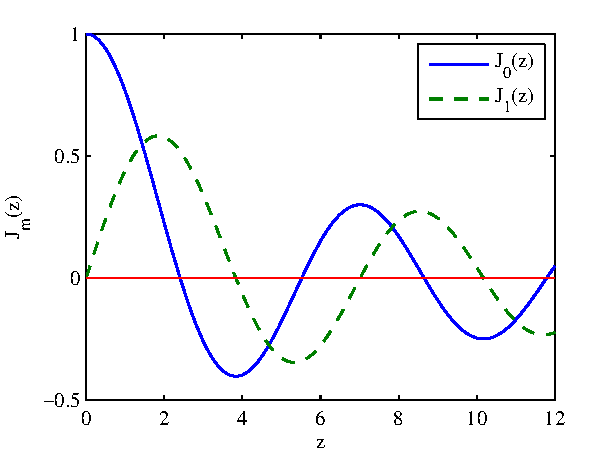
\includegraphics[width=\textwidth]{chp-2_bessel_j}
  \end{minipage}%
  \begin{minipage}[t]{0.5\textwidth}
    \centering
    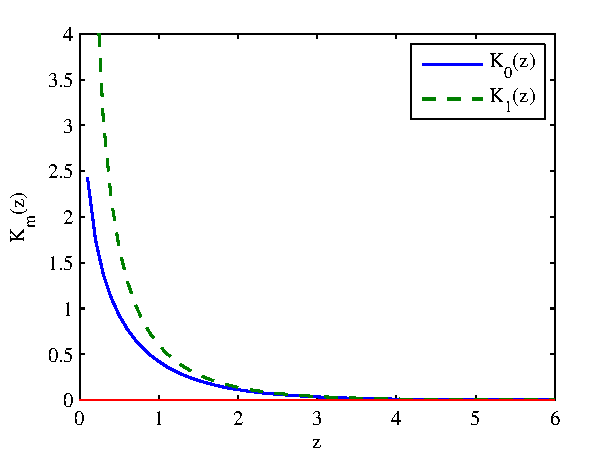
\includegraphics[width=\textwidth]{chp-2_bessel_k}
  \end{minipage}  \\
  \begin{minipage}[t]{0.5\textwidth}
    \centering
    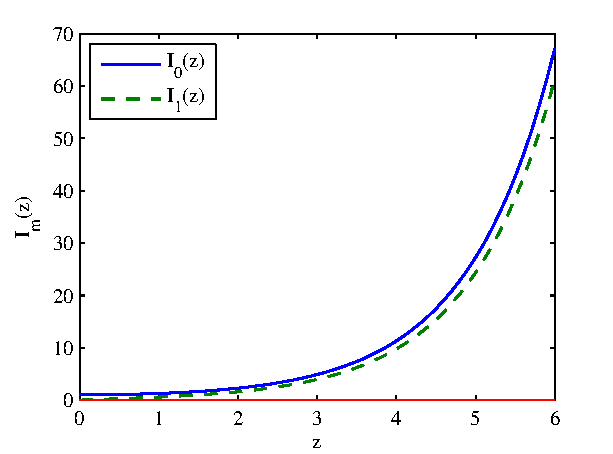
\includegraphics[width=\textwidth]{chp-2_bessel_i}
  \end{minipage}%
  \begin{minipage}[t]{0.5\textwidth}
    \centering
    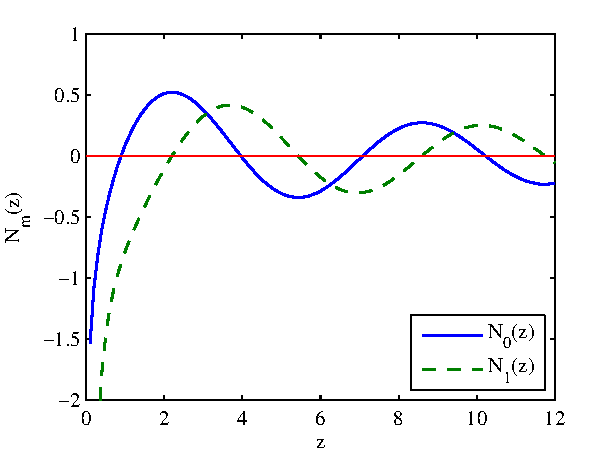
\includegraphics[width=\textwidth]{chp-2_bessel_n}
  \end{minipage}
\caption{贝塞尔函数}  \label{fig-bessel-function}
\end{figure}
其它类似的多个图形并排或者堆叠均可以灵活的运用minipage照猫画虎获得。

\section{图题}
其实上边的例子中已经包含了图题的引用命令\verb|\caption|。
例如图\ref{fig-bessel-function}中:
\begin{verbatim}
    \caption{贝塞尔函数}\label[fig-bessel-function]
\end{verbatim}
为当前的图形添加中文图题“贝塞尔函数”。同时添加标签“fig-bessel-function”。对图形的引用就是通过标签来实现的。

\section{图形的引用}
在已知图形的标签的基础之上,通过命令:
\begin{verbatim}
\ref{label}
\end{verbatim}
来引用标签为“label”的图形。\LaTeX 会自动将其替换为图形的编号。例如:
\begin{verbatim}
贝塞尔函数的图形如图\ref{fig-bessel-function}所示。
\end{verbatim}
的效果如下:\\
贝塞尔函数的图形如图\ref{fig-bessel-function}所示。

  % !Mode:: "TeX:UTF-8"
\chapter{表格}
\label{chap:table}

\section{普通三线表}
科技文献中常用的三线表:
\begin{table}[htbp]
 \centering\zihao{5}
 \caption{燕山大学硕士学位论文参考文献规则}\label{tab:ysubof}
 \begin{tabular}{llr}
 \toprule
    论文版本    & 参考文献标准    & 实施年份(年)  \\
 \midrule
    旧版        & BF7714-87       & 1987            \\
    新版        & GBT7714-2005    & 2005            \\
 \bottomrule
 \end{tabular}
\end{table}

实现代码如下:
\begin{verbatim}
\begin{table}[htbp]
 \centering\zihao{5}
 \caption{燕山大学硕士学位论文参考文献规则}\label{tab:ysubof}
 \begin{tabular}{llr}
 \toprule
    论文版本    & 参考文献标准    & 实施年份(年)  \\
 \midrule
    旧版        & BF7714-87       & 1987            \\
    新版        & GBT7714-2005    & 2005            \\
 \bottomrule
 \end{tabular}
\end{table}
\end{verbatim}

\section{有合并列的三线表}
合并列通常见于表格的第一行,在适当的位置使用\verb|\multicolumn| 命令即可。
\begin{table}[htbp]
\centering\zihao{5}
\caption{带有合并列的三线{\zihao{5}表}}\label{tab:test}
\begin{tabular}{llr} \toprule
\multicolumn{2}{c}{Item} \\ \cmidrule(r){1-2}
Animal & Description & Price (\$)\\ \midrule
Gnat & per gram & 13.65 \\
& each & 0.01 \\
Gnu & stuffed & 92.50 \\
Emu & stuffed & 33.33 \\
Armadillo & frozen & 8.99 \\ \bottomrule
\end{tabular}
\end{table}


该表格是采用如下代码实现的:
\begin{verbatim}
\begin{table}[htbp]
 \centering
 \caption{三线表}\label{tab:test}
 \begin{tabular}{llr}
 \toprule
    \multicolumn{2}{c}{Item}            \\
 \cmidrule(r){1-2}
    Animal  & Description   & Price (\$)\\
 \midrule
    Gnat    & per gram      & 13.65     \\
            & each          & 0.01      \\
    Gnu     & stuffed       & 92.50     \\
    Emu     & stuffed       & 33.33     \\
    Armadillo & frozen      & 8.99      \\
 \bottomrule
 \end{tabular}
\end{table}
\end{verbatim}

\section{表格的引用}
表格的引用同样是使用\verb|\ref{}| 命令实现的。例如“表\verb|\ref{tab:ysubof}|” 输出的结果为:表\ref{tab:ysubof}

  % !Mode:: "TeX:UTF-8"
\chapter{公式}
\label{chap:equ}
本章介绍基本公式的输入方法;矩阵和向量的输入;方程组的输入;多行公式的换行与对齐。
\LaTeX 中数学公式的输入依赖于数学环境。

在正文中用到的简短公式,可以直接使用两个美元符号“\$”括起来,如:
\begin{verbatim}
直角三角形三边长度满足关系式$a^2+b^2=c^2$
\end{verbatim}
得到的结果是:\\
直角三角形三边长度满足关系式$a^2+b^2=c^2$\\

而对于一些较为重要或者较复杂、需要编号的公式,则需要使用各种数学环境,例如使用equation环境:
\begin{verbatim}
\begin{equation}\label{chp-mode}
\mathbfit{E}=\mathrm{Re}(\mathbfit{E}(\mathbfit{r}))e^{j\omega t}
\end{equation}
\end{verbatim}
得到的结果是:
\begin{equation}\label{chp-mode}
\mathbfit{E}=\mathrm{Re}(\mathbfit{E}(\mathbfit{r}))e^{j\omega t}
\end{equation}
对它的引用方式为:\verb|公式\eqref{chp-mode}|\\
得到的结果为:公式\eqref{chp-mode}

如果不想对公式进行编号,则可以使用equation*环境:
\begin{verbatim}
\begin{equation*}\label{chp-m2}
\mathbfit{E}=\mathrm{Re}(\mathbfit{E}(\mathbfit{r}))e^{j\omega t}
\end{equation*}
\end{verbatim}
得到的结果是:
\begin{equation*}\label{chp-m2}
\mathbfit{E}=\mathrm{Re}(\mathbfit{E}(\mathbfit{r}))e^{j\omega t}
\end{equation*}

\section{上下标}
\verb|a_1+b^2\times c_1^2=0|输出结果为:$a_1+b^2\times c_1^2=0$

\section{分式}
命令\verb|\frac, \dfrac\ tfrac|可以用来输出分式:
\begin{verbatim}
\begin{equation}\label{fr}
  \sin\dfrac{\cos\dfrac{a}{b}}{c}=
  \sin\frac{\cos\frac{a}{b}}{c}=
  \sin\tfrac{\cos\tfrac{a}{b}}{c}
\end{equation}
\end{verbatim}
输出的结果是:
\begin{equation}\label{fr}
\sin\dfrac{\cos\dfrac{a}{b}}{c}=
\sin\frac{\cos\frac{a}{b}}{c}=
\sin\tfrac{\cos\tfrac{a}{b}}{c}
\end{equation}

当使用括号来括起纵向尺寸较大的对象例如分式时,要使用\verb|\left| 和
\verb|\right| 命令使括号在纵向上伸长。例如:
\begin{verbatim}
\begin{equation}\label{frr}
  \left(\frac{a}{b}\right)=(\frac{a}{b})
\end{equation}
\end{verbatim}
的输出结果是:
\begin{equation}\label{frr}
\left(\frac{a}{b}\right)=(\frac{a}{b})
\end{equation}

\section{矢量点乘与叉乘}
矢量点乘:\verb|$\mathbfit{A}\cdot\mathbfit{B}$|输出:$\mathbfit{A}\cdot\mathbfit{B}$

矢量叉乘:\verb|$\mathbfit{C}\times\mathbfit{D}$|输出:$\mathbfit{C}\times\mathbfit{D}$

\section{求和与积分}
命令\verb|\sum|和命令\verb|\int|负责输出求和与积分号。例如:
\begin{verbatim}
\begin{equation}\label{equ-sum}
  \sum_{i=1}^n\sin\beta_i^2=0
\end{equation}
\end{verbatim}
输出结果为:
\begin{equation}\label{equ-sum}
\sum_{i=1}^n\sin\beta_i^2=0
\end{equation}
\begin{verbatim}
\begin{equation}\label{equ-int}
  \int_a^b\frac{c}{d}\,\mathrm{d}x=0
\end{equation}
\end{verbatim}
输出结果为:
\begin{equation}\label{equ-int}
  \int_a^b\frac{c}{d}\,\mathrm{d}x=0
\end{equation}


\section{矩阵与数组}
矩阵与数组使用array环境:
\begin{verbatim}
\begin{equation}\label{equ-array}
  \left(
    \begin{array}{c} a \\ c \end{array}
  \right)=
  \left(
    \begin{array}{cc} a & b \\ c & d \end{array}
  \right)
\end{equation}
\end{verbatim}
输出结果是:
\begin{equation}\label{equ-array}
  \left(
  \begin{array}{c} a \\ c \end{array}
  \right)=
  \left(
  \begin{array}{cc} a & b \\ c & d \end{array}
  \right)
\end{equation}
也可以使用matrix环境:
\begin{verbatim}
\begin{equation}\label{equ-matrix}
  \begin{matrix} 0 & 1 \\ 1 & 0\end{matrix}=
  \begin{pmatrix}0 &-i \\ i & 0\end{pmatrix}=
  \begin{bmatrix}1 & 0 \\ 0 &-1\end{bmatrix}=
  \begin{vmatrix}a & b \\ c & d\end{vmatrix}
\end{equation}
\end{verbatim}
输出结果是:
\begin{equation}\label{equ-matrix}
  \begin{matrix} 0 & 1 \\ 1 & 0\end{matrix}=
  \begin{pmatrix}0 &-i \\ i & 0\end{pmatrix}=
  \begin{bmatrix}1 & 0 \\ 0 &-1\end{bmatrix}=
  \begin{vmatrix}a & b \\ c & d\end{vmatrix}
\end{equation}

\section{多行公式与对齐方法}
多行公式排列,每个公式都有自己的编号通常使用align环境。例如:
\begin{verbatim}
\begin{align}
  a_1+a_2+a_3 &=0 \label{equ-s1}\\
  b_1+b_2+b_3+b_4 &=0 \label{equ-s2}\\
  c_1+c_2 &=0 \label{equ-v1}
\end{align}
\end{verbatim}
输出结果为:
\begin{align}
  a_1+a_2+a_3 &=0 \label{equ-s1}\\
  b_1+b_2+b_3+b_4 &=0 \label{equ-s2}\\
  c_1+c_2 &=0 \label{equ-v1}
\end{align}
其中符号“\&”为对齐符号。这里实现了等号对齐。

\section{带有大括号的方程组}
与多行公式不同,方程组左侧使用“\verb|\left{|”加了一个大括号,另外只有一个公式编号,因此采用equation和aligned结合的方式,例如:
\begin{verbatim}
\begin{equation}\label{equ-fml}
  \left\{
  \begin{aligned}
    x^2+y^2 &=0\\
    x+y+z^2 &=0\\
    x^2+y+z &=0
  \end{aligned}
  \right.
\end{equation}
\end{verbatim}
输出结果为:
\begin{equation}\label{equ-fml}
  \left\{
  \begin{aligned}
    x^2+y^2 &=0\\
    x+y+z^2 &=0\\
    x^2+y+z &=0
  \end{aligned}
  \right.
\end{equation}


  % !Mode:: "TeX:UTF-8"
\chapter{参考文献}
\label{chap:bib}

所有被引用的参考文献信息均存储在模板目录中的“bib”目录下,文件名为“tex.bib”。
由于使用了BibTeX,参考文献的格式是不需要手动调整。模板中的ysubst.bst文件负责
文献格式输出。这里推荐您使用软件JabRef 来对文献进行管理。JabRef 支持中文,它可
以在这个网址下载到。\url{http://jabref.sourceforge.net/}

首先需要了解一个概念叫“BibTeX key”,也称作“BibTeX键”。它可以简单的理解为一篇
参考文献的“身份证号”。每一篇参考文献均有一个属于自己的不会重复的BibTeX key。
在引用文献的时候,需要使用引用命令\verb|\supercite{}|。

\section{单一参考文献}
例如这里我引用一篇文献:
\begin{verbatim}
P.Russell 是光子晶体光纤之父\supercite{Knight1996}
\end{verbatim}
其中“Knight1996”是我要引用的文献的BibTeX 键。输出的结果为:\\[5pt]
 P.Russell 是光子晶体光纤之父\supercite{Knight1996}\\[5pt]
 注意文献的编号是自动生成的,并且具有超链接功能。单击编号可以定位到文末的参考文献章节。

\section{多个连续参考文献}
 如果要一次引用多个文献,只要在引用命令中用英文逗号隔开各个BibTeX键即可,例如:
 \begin{verbatim}
我要引用2 篇文献\supercite{Knight1996,Knight2000}
\end{verbatim}
输出结果为: \\[5pt]
我要引用2 篇文献\supercite{Knight1996,Knight2000}


如果是3 篇或者以上,加入更多BibTeX 键即可。例如:
 \begin{verbatim}
3 篇文献\supercite{Knight1996,Knight2000,Knight2002}
\end{verbatim}
输出结果为: \\[5pt]
3 篇文献\supercite{Knight1996,Knight2000,Knight2002}

更多文献的例子:
 \begin{verbatim}
很多很多文献\supercite{Kivshar2008,John1987,Jing2010,Jeon2005,%
Jastrow2008,Jackson2008,Huttunen2005,Hou2008,Hilligsoe2004,%
Hassani2008,Han2002}
\end{verbatim}

输出的结果为:很多很多文献\supercite{Kivshar2008,John1987,Jing2010,Jeon2005,%
Jastrow2008,Jackson2008,Huttunen2005,Hou2008,Hilligsoe2004,%
Hassani2008,Han2002}



\section{多个不连续参考文献}
 \begin{verbatim}
四个不连续文献\supercite{Zhu2004,Zhu2001,Yin2011,Knight1996}
\end{verbatim}
四个不连续文献\supercite{Zhu2004,Zhu2001,Yin2011,Knight1996}

  % !Mode:: "TeX:UTF-8"
\chapter{插入程序代码}
\label{chap:chap-5}

使用lisitings宏包可以在正文中插入程序的代码,插入的代码有自己的字体,可以实现行号、关键字高亮等功能。该环境的参数language决定了程序
的类型,例如\verb|language={[77]Fortran}|指定程序代码为FORTRAN语言;\verb|language={MATLAB}|指定程序代码为MATLAB的m语言。下边给出具体的例子。

\section{FORTRAN}
\begin{verbatim}
\begin{lstlisting}[language={[77]Fortran},
numbers=left,
numberstyle=\tiny,
basicstyle=\small\ttfamily,
stringstyle=\color{purple},
keywordstyle=\color{blue}\bfseries,
commentstyle=\color{brown},
frame=single]
C MATLAB gateway
      subroutine mexFunction(nlhs, plhs, nrhs, prhs)
C variables
      integer nlhs, nrhs
      integer plhs(*), prhs(*)
C input pointers
      pr_x=mxgetpr(prhs(1))
      pr_x1=mxgetpr(prhs(2))
C output pointers
      plhs(1)=mxCreateDoubleScalar(0)
      pr_y=mxGetPr(plhs(1))
C calculation
      call eim(%val(pr_x),%val(pr_x1),%val(pr_y))
      end subroutine mexFunction
\end{lstlisting}
\end{verbatim}
输出的结果为:
\begin{lstlisting}[language={[77]Fortran},
numbers=left,
numberstyle=\tiny,
basicstyle=\small\ttfamily,
stringstyle=\color{purple},
keywordstyle=\color{blue}\bfseries,
commentstyle=\color{brown},
frame=single]
C MATLAB gateway
      subroutine mexFunction(nlhs, plhs, nrhs, prhs)
C variables
      integer nlhs, nrhs
      integer plhs(*), prhs(*)
C input pointers
      pr_x=mxgetpr(prhs(1))
      pr_x1=mxgetpr(prhs(2))
C output pointers
      plhs(1)=mxCreateDoubleScalar(0)
      pr_y=mxGetPr(plhs(1))
C calculation
      call eim(%val(pr_x),%val(pr_x1),%val(pr_y))
      end subroutine mexFunction
\end{lstlisting}

\section{MATLAB}
\begin{verbatim}
\begin{lstlisting}[language={MATLAB},
numbers=left,
numberstyle=\tiny,
basicstyle=\small\ttfamily,
stringstyle=\color{purple},
keywordstyle=\color{blue}\bfseries,
commentstyle=\color{brown},
frame=single]
% bessel j

n=-0:0.1:12;
y=n*0;
b0n=besselj(0,n);
b1n=besselj(1,n);
plot(n,b0n,'-',n,b1n,'-',0:0.1:12,y)

ylabel('J_m(z)')
xlabel('z')
legend('J_0(z)','J_1(z)')
\end{lstlisting}
\end{verbatim}
输出的结果为:
\begin{lstlisting}[language={MATLAB},
numbers=left,
numberstyle=\tiny,
basicstyle=\small\ttfamily,
stringstyle=\color{purple},
keywordstyle=\color{blue}\bfseries,
commentstyle=\color{brown},
frame=single]
% bessel j

n=-0:0.1:12;
y=n*0;
b0n=besselj(0,n);
b1n=besselj(1,n);
plot(n,b0n,'-',n,b1n,'-',0:0.1:12,y)

ylabel('J_m(z)')
xlabel('z')
legend('J_0(z)','J_1(z)')
\end{lstlisting}

\section{C++}
\begin{verbatim}
\begin{lstlisting}[language={C++},
numbers=left,
numberstyle=\tiny,
basicstyle=\small\ttfamily,
stringstyle=\color{purple},
keywordstyle=\color{blue}\bfseries,
commentstyle=\color{brown},
frame=single]
# include{iostream.h}
void main()
int r;
double n;
{
cout<<"hello, LaTeX!"<<endl;
}
\end{lstlisting}
\end{verbatim}
输出的结果为:
\begin{lstlisting}[language={C++},
numbers=left,
numberstyle=\tiny,
basicstyle=\small\ttfamily,
stringstyle=\color{purple},
keywordstyle=\color{blue}\bfseries,
commentstyle=\color{brown},
frame=single]
# include{iostream.h}
void main()
int r;
double n;
{
cout<<"hello, LaTeX!"<<endl;
}
\end{lstlisting}

  % !Mode:: "TeX:UTF-8"
\chapter{数字物理量与单位}
\label{chap:unit}
模板加载了siunitx 宏包,可以实现长串数字位数的正确分割和各种物理量单位的自动格式化,避免
手工调用数学环境输入单位。尤其适用于理工科各种物理量的输入。该宏包的引入主要是为了解决论文
格式标准中的这个要求:
数字的书写不必每格一个数码,一般每两数码占一格,数字间分节不用分位号",",\emph{凡4位或4位以上的数都从个位起每3位数空\textbf{半个数码(1/4汉字)}。“\num{3 000000}”,不要写成}“3,000,000”,\emph{小数点后的数从小数点起向右按\textbf{每三位一组分节}。一个用阿拉伯数字书写的多位数不能从数字中间转行。}

\section{数字}
使用\verb|\num| 命令可以输入正确格式的长数字,包括科学计数法格式的数字。

\begin{table}[htbp]
\centering\zihao{5}
\caption{siunitx 宏包与\LaTeX 数学环境输出效果对比}
\begin{tabular}{ll|ll}
\toprule
siunitx 输出样式    & siunitx 输入方式          & \LaTeX 数学环境输出样式  & \LaTeX 数学环境输入方式     \\
\midrule
\num{123456789}     & \verb|\num{123456789}|    & 123456789             & \verb|123456789|         \\
\num{-1000000}      & \verb|\num{-1000000}|     & $-1000000$            & \verb|$-1000000$|        \\
\num{3.2e-8}        & \verb|\num{3.2e-8}|       & $3.2\times 10^{-8}$   & \verb|$3.2\times 10^{-8}$|\\
\num{1.2345678}     & \verb|\num{1.2345678}|    & 1.2345678             & \verb|1.2345678|          \\
\bottomrule
\end{tabular}
\end{table}

\section{单位}
单独输入单位时,可以采用\verb|\si|命令。

\begin{table}[htbp]
\centering\zihao{5}
\caption{单位的不同输入方式}
\begin{tabular}{ll}
\toprule
输出样式  &输入方式     \\
\midrule
\si{kg.m/s^2}                           & \verb|\si{kg.m/s^2}|         \\
\si{g_{polymer}mol_{cat}.s^{-1}}       & \verb|\si{g_{polymer}mol_{cat}.s^{-1}}|\\
\si{\kilo\gram\metre\per\square\second} & \verb|\si{\kilo\gram\metre\per\square\second}|\\
\si{\gram\per\cubic\centi\metre}        &\verb|\si{\gram\per\cubic\centi\metre}|\\
\si{\square\volt\cubic\lumen\per\farad} &\verb|\si{\square\volt\cubic\lumen\per\farad}|\\
\si{\metre\squared\per\gray\cubic\lux}  &\verb|\si{\metre\squared\per\gray\cubic\lux}|\\
\si{\henry\second}                      &\verb|\si{\henry\second}|\\
\bottomrule
\end{tabular}
\end{table}

\section{同时输入数字与单位}

通常情况下,数字与单位是共同给出的,这时可以采用\verb|\SI| 命令。注意这里的 SI 是大写的。并且加入不同的可选项,最终的效果也不同。

\begin{table}[htbp]
\centering\zihao{5}
\caption{同时输入数字与单位}
\begin{tabular}{ll}
\toprule
输出样式    & 输入方式  \\
\midrule
\SI[mode=text]{1.23}{J.mol^{-1}.K^{-1}}         & \verb|\SI[mode=text]{1.23}{J.mol^{-1}.K^{-1}}| \\
\SI{.23e7}{\candela}                            & \verb|\SI{.23e7}{\candela}|\\
\SI[per-mode=symbol]{1.99}[\$]{\per\kilogram}   & \verb|\SI[per-mode=symbol]{1.99}[\$]{\per\kilogram}|\\
\SI[per-mode=fraction]{1,345}{\coulomb\per\mole}& \verb|\SI[per-mode=fraction]{1,345}{\coulomb\per\mole}|\\
\bottomrule
\end{tabular}
\end{table}

\section{附1:国际标准单位与导出单位输入方式}

\begin{table}[htbp]
\centering\zihao{5}
\caption{国际标准单位输入方式}
\begin{tabular}{lllp{10pt}lll}
\toprule
单位    & 命令  & 符号  &   & 单位    & 命令  & 符号  \\
\midrule
安培    & \verb|\ampere|    & \si{\ampere}   && 坎德拉  & \verb|\candela|   & \si{\candela}  \\
开尔文  & \verb|\kelvin|    & \si{\kelvin}   && 千克    & \verb|\kilogram|  & \si{\kilogram}    \\
米      & \verb|\meter|     & \si{\meter}    && 摩尔    & \verb|\mole|      & \si{\mole}    \\
秒      & \verb|\second|    & \si{\second}   &&     &        &      \\
\bottomrule
\end{tabular}
\end{table}

\begin{table}[htbp]
\centering\zihao{5}
\caption{国际标准导出单位输入方式}
\begin{tabular}{lllp{10pt}lll}
\toprule
单位    & 命令  & 符号  &   & 单位    & 命令  & 符号  \\
\midrule
becquerel       & \verb|\becquerel|     & \si{\becquerel}       & & newton      & \verb|\newton|    & \si{\newton} \\
degree Celsius  & \verb|\degreeCelsius| & \si{\degreeCelsius}   & & ohm         & \verb|\ohm|       & \si{\ohm}\\
coulomb         & \verb|\coulomb|       & \si{\coulomb}         & & pascal      & \verb|\pascal|    & \si{\pascal}\\
farad           & \verb|\farad|         & \si{\farad}           & & radian      & \verb|\radian|    & \si{\radian} \\
gray            & \verb|\gray|          & \si{\gray}            & & siemens     & \verb|\siemens|   & \si{\siemens}    \\
hertz           & \verb|\hertz|         & \si{\hertz}           & & sievert     & \verb|\sievert|   & \si{\sievert}\\
henry           & \verb|\henry|         & \si{\henry}           & & steradian   & \verb|\steradian| & \si{\steradian}\\
joule           & \verb|\joule|         & \si{\joule}           & & tesla       & \verb|\tesla|     & \si{\tesla}\\
katal           & \verb|\katal|         & \si{\katal}           & & volt        & \verb|\volt|      & \si{\volt}\\
lumen           & \verb|\lumen|         & \si{\lumen}           & & watt        & \verb|\watt|      & \si{\watt}\\
lux             & \verb|\lux|           & \si{\lux}             & & weber       & \verb|\weber|     & \si{\weber}\\
\bottomrule
\end{tabular}
\end{table}
\section{附2:国际标准单位前缀}

\begin{table}[htbp]
\centering\zihao{5}
\caption{国际标准单位前缀输入方式}
\begin{tabular}{llllp{10pt}llll}
\toprule
名称    & 命令          & 符号          & 指数  &   & 名称      & 命令          & 符号      & 指数 \\
\midrule
yocto   & \verb|\yocto| & \si{\yocto}   & -24   &   & deca      &\verb|\deca|   &\si{\deca} & 1     \\
zepto   & \verb|\zepto| & \si{\zepto}   & -21   &   & hecto     &\verb|\hecto|  &\si{\hecto}& 2\\
atto    & \verb|\atto|  & \si{\atto}    & -18   &   & kilo      &\verb|\kilo|   &\si{\kilo} & 3\\
femto   & \verb|\femto| & \si{\femto}   & -15   &   & mega      &\verb|\mega|   &\si{\mega} & 6\\
pico    & \verb|\pico|  & \si{\pico}    & -12   &   & giga      &\verb|\giga|   &\si{\giga} & 9\\
nano    & \verb|\nano|  & \si{\nano}    & -9    &   & tera      &\verb|\tera|   &\si{\tera} & 12\\
micro   & \verb|\micro| & \si{\micro}   & -6    &   & peta      &\verb|\peta|   &\si{\peta} & 15\\
milli   & \verb|\milli| & \si{\milli}   & -3    &   & exa       &\verb|\exa|    &\si{\exa}  & 18\\
centi   & \verb|\centi| & \si{\centi}   & -2    &   & zetta     &\verb|\zetta|  &\si{\zetta}& 21\\
deci    & \verb|\deci|  & \si{\deci}    & -1    &   & yotta     &\verb|\yotta|  &\si{\yotta}& 24\\
\bottomrule
\end{tabular}
\end{table}

  % !Mode:: "TeX:UTF-8"
\begin{conclusion}
\label{chap:conclusion}

结论作为学位论文正文的组成部分,单独排写,不加章标题序号,不标注引用文献。结论内容一般在2000字以内。

结论应是作者在学位论文研究过程中所取得的创新性成果的概要总结,不能与摘要混为一谈。结论应包括论文的主要结果、创新点、展望三部分,在结论中应概括论文的核心观点,明确、客观地指出本研究内容的创新性成果(含新见解、新观点、方法创新、技术创新、理论创新),并指出今后进一步在本研究方向进行研究工作的展望与设想。对所取得的创新性成果应注意从定性和定量两方面给出科学、准确的评价,分(1)、(2)、(3)…条列出,宜用“提出了”、“建立了”等词叙述。此外,结论的撰写还应符合以下基本要求:

(1)结论具有相对的独立性,不应是对论文中各章小结的简单重复。结论要与引言相呼应,以自身的条理性、明确性、客观性反映论文价值。对论文创新内容的概括,评价要适当。

(2)结论措辞要准确、严谨,不能模棱两可,避免使用“大概”、“或许”、“可能是”等词语。结论中不应有解释性词语,而应直接给出结果。结论中一般不使用量的符号,而宜用量的名称。

(3)结论应指出论文研究工作的局限性或遗留问题,如条件所限,或存在例外情况,或本论文尚难以解释或解决的问题。

(4)常识性的结果或重复他人的结果不应作为结论。

\end{conclusion} 

  %% 附录
  %\appendix
  %%%%%%%%%%%%%%%%%%%%%% appendix.tex %%%%%%%%%%%%%%%%%%%%%%%%%%%%%%%%%
%
% sample appendix
%
% Use this file as a template for your own input.
%
%%%%%%%%%%%%%%%%%%%%%%%% Springer-Verlag %%%%%%%%%%%%%%%%%%%%%%%%%%

\chapter{Chapter Heading}
\label{introA} % Always give a unique label
% use \chaptermark{}
% to alter or adjust the chapter heading in the running head

Use the template \emph{appendix.tex} together with the Springer document class SVMono (monograph-type books) or SVMult (edited books) to style appendix of your book in the Springer layout.


\section{Section Heading}
\label{sec:A1}
% Always give a unique label
% and use \ref{<label>} for cross-references
% and \cite{<label>} for bibliographic references
% use \sectionmark{}
% to alter or adjust the section heading in the running head
Instead of simply listing headings of different levels we recommend to let every heading be followed by at least a short passage of text. Further on please use the \LaTeX\ automatism for all your cross-references and citations.


\subsection{Subsection Heading}
\label{sec:A2}
Instead of simply listing headings of different levels we recommend to let every heading be followed by at least a short passage of text. Further on please use the \LaTeX\ automatism for all your cross-references and citations as has already been described in Sect.~\ref{sec:A1}.

For multiline equations we recommend to use the \verb|eqnarray| environment.
\begin{eqnarray}
\vec{a}\times\vec{b}=\vec{c} \nonumber\\
\vec{a}\times\vec{b}=\vec{c}
\label{eq:A01}
\end{eqnarray}

\subsubsection{Subsubsection Heading}
Instead of simply listing headings of different levels we recommend to let every heading be followed by at least a short passage of text. Further on please use the \LaTeX\ automatism for all your cross-references and citations as has already been described in Sect.~\ref{sec:A2}.

Please note that the first line of text that follows a heading is not indented, whereas the first lines of all subsequent paragraphs are.

% For figures use
%
\begin{figure}[t]
\sidecaption[t]
% Use the relevant command for your figure-insertion program
% to insert the figure file.
% For example, with the graphicx style use
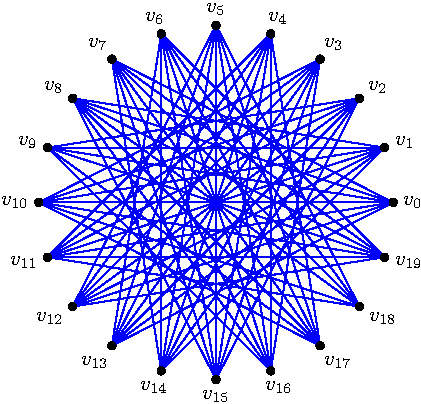
\includegraphics[scale=.65]{figure}
%
% If no graphics program available, insert a blank space i.e. use
%\picplace{5cm}{2cm} % Give the correct figure height and width in cm
%
\caption{Please write your figure caption here}
\label{fig:A1}       % Give a unique label
\end{figure}

% For tables use
%
\begin{table}
\caption{Please write your table caption here}
\label{tab:A1}       % Give a unique label
%
% Follow this input for your own table layout
%
\begin{tabular}{p{2cm}p{2.4cm}p{2cm}p{4.9cm}}
\hline\noalign{\smallskip}
Classes & Subclass & Length & Action Mechanism  \\
\noalign{\smallskip}\hline\noalign{\smallskip}
Translation & mRNA$^a$  & 22 (19--25) & Translation repression, mRNA cleavage\\
Translation & mRNA cleavage & 21 & mRNA cleavage\\
Translation & mRNA  & 21--22 & mRNA cleavage\\
Translation & mRNA  & 24--26 & Histone and DNA Modification\\
\noalign{\smallskip}\hline\noalign{\smallskip}
\end{tabular}
$^a$ Table foot note (with superscript)
\end{table}
%



% 以下为附件部分
%----------------------------%
\backmatter

  % 参考文献
  %|- 使用 BibTeX
    \bibliography{bib/tex}
    %\nocite{*}
  %|-不使用 BibTeX
    %
\begin{thebibliography}{10}

\bibitem{deng:01a}
{�˽���,~��ȽȽ,~�³���}.
\newblock {\em \LaTeXe{}~�Ƽ��Ű�ָ��}.
\newblock ��ѧ������,~���:~7-03-009239-2/TP.1516, ����, 2001.

\bibitem{wang:00a}
����.
\newblock {\em \LaTeXe{}~��ͼָ��}.
\newblock 2000.

\bibitem{zhang:03a}
���ֲ�.
\newblock {\em �����°�~CCT~��˵��}.
\newblock 2003.

\bibitem{lshort-cn}
C\TeX{} ������.
\newblock {\em lshort~����~3.20}.
\newblock 2003.

\bibitem{knuth86e}
Donald~E. Knuth.
\newblock {\em Computer Modern Typefaces}, volume~E of {\em Computers and
  Typesetting}.
\newblock Addison-Wesley, Reading, Massachusetts, 1986.

\bibitem{knuth86d}
Donald~E. Knuth.
\newblock {\em {METAFONT}: The Program}, volume~D of {\em Computers and
  Typesetting}.
\newblock Addison-Wesley, Reading, Massachusetts, 1986.

\bibitem{knuth86c}
Donald~E. Knuth.
\newblock {\em The {METAFONT}book}, volume~C of {\em Computers and
  Typesetting}.
\newblock Addison-Wesley, Reading, Massachusetts, 1986.

\bibitem{knuth86b}
Donald~E. Knuth.
\newblock {\em {TeX}: The Program}, volume~B of {\em Computers and
  Typesetting}.
\newblock Addison-Wesley, Reading, Massachusetts, 1986.

\bibitem{knuth86a}
Donald~E. Knuth.
\newblock {\em The {TeX}book}, volume~A of {\em Computers and Typesetting}.
\newblock Addison-Wesley, Reading, Massachusetts, 1986.

\bibitem{lamport85a}
Leslie Lamport.
\newblock {\em {LaTeX} --- A Document Preparation System: User's Guide and
  Reference Manual}.
\newblock Addison-Wesley, Reading, Massachusetts, 2nd edition, 1985.

\end{thebibliography}


  % 发表文章目录
  % !Mode:: "TeX:UTF-8"
\begin{achievement}

\project
\begin{enumerate}\setlength{\itemsep}{0pt}
\renewcommand{\labelenumi}{[\theenumi]}
\item ×××,×××.人足机构学仿生与生物融合机构系统研究, 国家自然科学基金资助项目. 课题编号:50675191.
\item ×××,×××.双重驱动少自由度并联机构型综合理论与应用, 河北省自然科学基金资助项目. 课题编号:E2009000388.
\item $\cdots$
\end{enumerate}
\publications
\begin{enumerate}\setlength{\itemsep}{0pt}
\renewcommand{\labelenumi}{[\theenumi]}
\item ×××, ××× and ×××. Optimization of Dispersion Properties of Photonic Crystal Fibers Using a Real-Coded Genetic Algorithm[J]. Chin. Phys. Lett., 2011, 28 (6): 064215
\item ×××,×××.并联2-RRR/UPRR踝关节康复机器人机构及其运动学[J]. 机器人, 2010, 32(1):6-12 .(EI收录号: 20101212786168)
\item $\cdots$
\end{enumerate}

{\noindent\textbf{(三)申请及已获得的专利}}    % 无专利时此项不必列出
\begin{enumerate}\setlength{\itemsep}{0pt}
\renewcommand{\labelenumi}{[\theenumi]}
\item ×××,×××.具有远程运动中心的三自由度转动并联机构:中国, 200910073844.8 [P]. 2011-01-05.
\item ×××,×××. 五自由度双重驱动并联机构:中国, 200910075071.7 [P]. 2011-01-05.
\end{enumerate}

{\noindent\textbf{(四)科研获奖}}    % 无奖励时此项不必列出
\begin{enumerate}\setlength{\itemsep}{0pt}
\renewcommand{\labelenumi}{[\theenumi]}
\item ×××,×××. 机器人机型综合及结构分析理论. XX省科学技术二等奖, 2009.
\end{enumerate}
\end{achievement} 

  % 致谢
  % !TEX root = ../main.tex
\begin{thanks}

感谢原中科大本硕博论文模版的制作人员

包括但不限于ywg,XPS,Liuqs,Guolicai,刘青松等原模版的制作者和维护者

我在这里只是按照中国地质大学的work版本的硕士论文模版进行了一定的修改

以满足使用\LaTeX 撰写中国地质大学硕士论文的目的

感谢大家对本模板更新工作的支持!

本模板以及本示例文档还存在许多不足之处,欢迎大家测试并及时提供反馈。

\begin{flushright}
seeksky@CUG

欢迎访问我的博客 http://jinlaixu.net
\end{flushright}


在中国地质大学完成本科和硕士连读学业的七年里,我所从事的学习和研究工作,都是在导师以及系里其他老师和同学的指导和帮助下进行的。在完成论文之际,请容许我对他们表达诚挚的谢意。

首先感谢导师XXX教授和XXX副教授多年的指导和教诲,是他们把我带到了计算机视觉的研究领域。X老师严谨的研究态度及忘我的工作精神,X老师认真细致的治学态度及宽广的胸怀,都将使我受益终身。

感谢班主任XXX老师和XX老师多年的关怀。感谢XXX、XX、XX等老师,他们本科及研究生阶段的指导给我研究生阶段的研究工作打下了基础。

感谢XX、XXX、XXX、XX、XXX、XXX、XXX、XX等师兄师姐们的指点和照顾;感谢XXX、XX、XXX等几位同班同学,与你们的讨论使我受益良多;感谢XXX、XX、XXX、XX、XXX等师弟师妹,我们在XXX实验室共同学习共同生活,一起走过了这段愉快而难忘的岁月。

感谢科大,感谢一路走过来的兄弟姐妹们,在最宝贵年华里,是你们伴随着我的成长。

最后,感谢我家人一贯的鼓励和支持,你们是我追求学业的坚强后盾。

\vskip 18pt

\begin{flushright}

~~~~赵钱孙~~~~

\today

\end{flushright}

\end{thanks}


  % 作者简介
  \resumeitem{个人简历:}
\noindent xxxx 年 xx 月 xx 日出生于 xx 省 xx 县。\\
\noindent xxxx 年 9 月考入 xx 大学 xx 系 xx 专业,xxxx 年 7 月本科毕业并获得 xx 学士学位。\\
\noindent xxxx 年 9 月免试进入 xx 大学 xx 系攻读 xx 学位至今。

\resumeitem{发表论文:} % 发表的和录用的合在一起
\begin{enumerate}[{[}1{]}]
\item Yang Y, Ren T L, Zhang L T, et al. Miniature microphone with silicon-
  based ferroelectric thin films. Integrated Ferroelectrics, 2003,
  52:229-235. (SCI 收录, 检索号:758FZ.)
\item 杨轶, 张宁欣, 任天令, 等. 硅基铁电微声学器件中薄膜残余应力的研究. 中国机
  械工程, 2005, 16(14):1289-1291. (EI 收录, 检索号:0534931 2907.)
\item 杨轶, 张宁欣, 任天令, 等. 集成铁电器件中的关键工艺研究. 仪器仪表学报,
  2003, 24(S4):192-193. (EI 源刊.)
\item Yang Y, Ren T L, Zhu Y P, et al. PMUTs for handwriting recognition. In
  press. (已被 Integrated Ferroelectrics 录用. SCI 源刊.)
\item Wu X M, Yang Y, Cai J, et al. Measurements of ferroelectric MEMS
  microphones. Integrated Ferroelectrics, 2005, 69:417-429. (SCI 收录, 检索号
  :896KM.)
\item 贾泽, 杨轶, 陈兢, 等. 用于压电和电容微麦克风的体硅腐蚀相关研究. 压电与声
  光, 2006, 28(1):117-119. (EI 收录, 检索号:06129773469.)
\item 伍晓明, 杨轶, 张宁欣, 等. 基于MEMS技术的集成铁电硅微麦克风. 中国集成电路, 
  2003, 53:59-61.
\end{enumerate}

\resumeitem{研究成果:} % 有就写,没有就删除
\begin{enumerate}[{[}1{]}]
\item 任天令, 杨轶, 朱一平, 等. 硅基铁电微声学传感器畴极化区域控制和电极连接的
  方法: 中国, CN1602118A. (中国专利公开号.)
\item Ren T L, Yang Y, Zhu Y P, et al. Piezoelectric micro acoustic sensor
  based on ferroelectric materials: USA, No.11/215, 102. (美国发明专利申请号.)
\end{enumerate}



\end{document}
%%===========================%
%% 全文结束
